% -*- coding: UTF-8 -*-
% vim: autoindent expandtab tabstop=4 sw=4 sts=4 filetype=tex
% vim: spelllang=de spell
% chktex-file 27 - disable warning about missing include files

\section{Domänenmodell}
\label{sec:domain-model}

Der wesentliche Schritt der objektorientierten Analyse ist die Zerlegung einer
Domäne in essentielle Konzepte oder Objekte~\cite[S. 134]{larman_applying_2004}.

In UML wird ein Domänenmodell typischerweise als eine Menge von
Klassendiagrammen ohne Operationen dargestellt. Es liefert eine konzeptuelle
Perspektive und kann folgende Elemente beinhalten~\cite[S. 134]{larman_applying_2004}:
\begin{itemize}
    \item{Objekte der Domäne oder konzeptuelle Klassen}
    \item{Relationen zwischen konzeptuellen Klassen}
    \item{Attribute der konzeptuellen Klassen}
\end{itemize}

\citeauthor{larman_applying_2004} weist darauf hin, dass nicht versucht werden
sollte von Beginn weg ein möglichst genaues, vollständiges oder ``korrektes''
Domänenmodell zu erstellen. Ein solcher Ansatz führt zu ``analysis paralysis''
und sollte daher vermieden werden, da dies wenig bis keinen Mehrwert
bring~\cite[S. 133]{larman_applying_2004}.

Da angedacht ist, dass die Software aus zwei Applikationen, dem
\textit{Player} sowie dem \textit{Editor}, besteht, wird für jede
Applikation ein Domänenmodell erstellt.

\subsection{Player}
\label{subsec:domain-model:player}

Abbildung~\ref{fig:domain-model:player} zeigt das Domänenmodell der
Player-Applikation. Das Modell ist bewusst minimal gehalten und zeigt nur die
nötigsten Komponenten. Im Zentrum steht das Player-Objekt. Dieses liest ein
DemoScript, welches eine exportierte Echtzeit-Animation des Editors darstellt.
Ausgehend vom DemoScript kann schliesslich der Hauptknoten des Graphen gefunden
evaluiert werden. Ausgehend von diesem wird so die gesamte Echtzeit-Animation
aufgebaut und wiedergeben. DemoData dient der Verwaltung von DemoScript, also
zum Export von diesem.

Viele essentielle Konzepte beziehungsweise Objekte fehlen in diesem Modell
bewusst. Diese werden während den Iterationen der darauffolgenden Projektarbeit
erarbeitet. Ein Teil davon findet sich im Domänenmodell des Editors
(siehe~\autoref{subsec:domain-model:editor}) sowie im Klassendiagramm des Prototypen
(siehe~\autoref{chap:prototype}).

\begin{figure}[H]
    \centering
    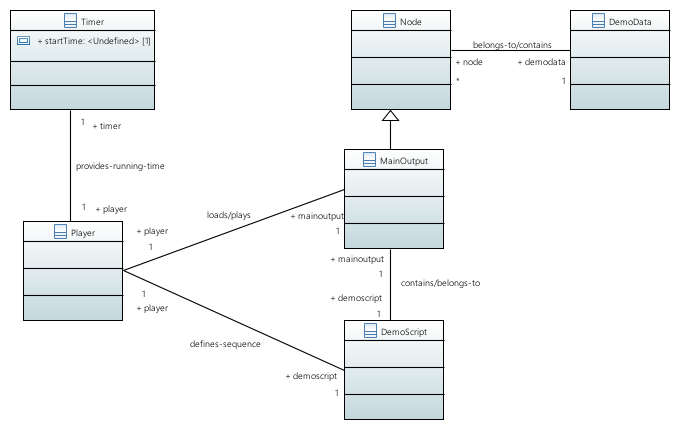
\includegraphics{img/player_domain_model.pdf}
    \caption{Domänenmodell der
        Player-Applikation}\label{fig:domain-model:player}
\end{figure}

\subsection{Editor}
\label{subsec:domain-model:editor}

Abbildung~\ref{fig:domain-model:editor} zeigt das Domänenmodell der
Editor-Applikation. Analog dem vorherigen Modell steht hier das Editor-Objekt
im Zentrum. Dieses bildet die Schnittstelle zwischen der grafischen
Benutzeroberfläche (GUI) und der Applikationslogik.

Die Komponenten der grafischen Benutzeroberfläche wurden in diesem Modell
bewusst weggelassen, da dies das Modell nur unnötig vergrössern würde. Die
eigentliche Logik findet sich in den essentiellen Konzepten beziehungsweise in
den hier gezeigten Objekten. Die grafische Benutzeroberfläche bildet diese nur
ab respektive Kopien davon.

Im mittleren Teil ist mit dem Node-Objekt und dessen Spezialisierung die
gesamte Struktur des Graphen angedeutet. Dies werden schliesslich die Objekte
sein, welche ein Anwender nutzen kann um Echtzeit-Animationen zu erstellen.

Im rechten Teil des Modelles stellen die Objekte Parameter, Keyframe,
TimelineClip und Timeline Elemente zur Animation dar. Pro Parameter kann zu
einem bestimmten Zeitpunkt der Zeitachse ein Schlüsselbild (Keyframe) gesetzt
werden. Timeline stellt die gesamte Zeitachse und TimelineClip einzelne
Elemente dieser dar. Es handelt sich bei Letzteren um Szenen.

Auch hier fehlen wiederum etliche Details, wie zum Beispiel das gesamte
Rendering inklusive den Shadern. Ein Teil davon ist wiederum im Klassendiagramm
des Prototypen (siehe~\autoref{chap:prototype}) ersichtlich.

Wie Eingangs erwähnt, ist es nicht das Ziel ein vollständiges oder
``korrektes'' Domänenmodell zu erstellen. Es geht viel mehr um einen ersten
Anstoss zur eigentlichen Implementierung. Alle weiteren Details werden während
den Iterationen der darauffolgenden Projektarbeit erarbeitet.

\begin{figure}[H]
    \centering
    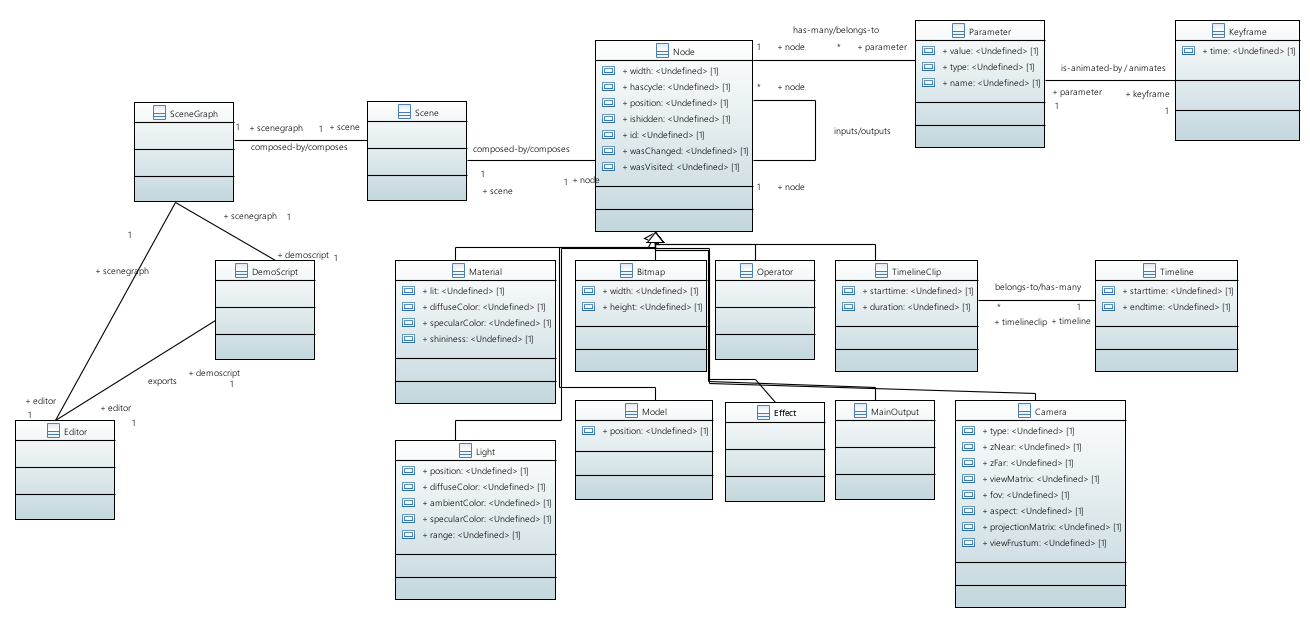
\includegraphics[angle=90,width=0.8\textwidth]{img/editor_domain_model.pdf}
    \caption{Domänenmodell der
        Editor-Applikation}\label{fig:domain-model:editor}
\end{figure}
